\documentclass[10pt,a4paper]{article}
\usepackage[utf8]{inputenc}
\usepackage{amsmath}
\usepackage{amsfonts}
\usepackage{amssymb}
\usepackage{graphicx}
\author{Pranav Satheesh}
\title{Relativity Assignments}
\begin{document}
\maketitle

\section{Einstein's velocity addition}

In this problem, you will derive the velocity addition rule in relativity using Lorentz transformations. Consider a particle A in the frame B. Her velocity w.r.t frame B is $V_{AB}$. In another frame C moving w.r.t B with a velocity $V_{CB}$. Show that the velocity of A w.r.t to the frame C using \textbf{Lorentz transformation}:

\begin{equation}
V_{AC} = \frac{V_{AB} + V_{BC}}{1 + (V_{AB} V_{BC} / c^2)}
\end{equation}

(\textit{\textbf{Hint} : You can use consider the velocity to be $u =\frac{dx}{dt}$ in the frame B and then write the lorentz transformation equations for $dx$ and $dt$ to the frame C where these become $\bar{dx}$ and $\bar{dt}$})

\section{Superluminal Motion}
Astronomers observed radio galaxies moving with velocities exceeding the velocity of c!
M87 is an example in the Virgo cluster
The distance to this galaxy, M87, is about D = 62 million light years. One can use this distance to convert angular separations into linear separations across the line of sight. 


\begin{figure}[htbp]
\centering
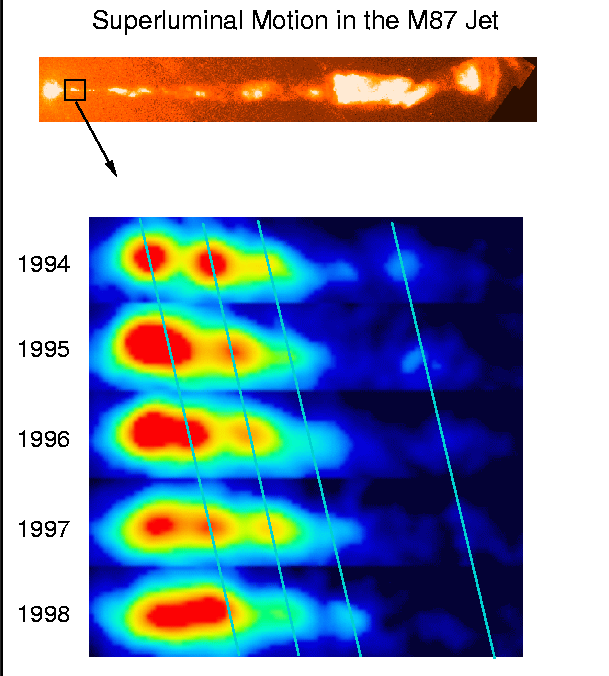
\includegraphics[scale=0.25]{lum1.png} 
\caption{Blobs}
\end{figure}
Now, look at one of the blobs: the innermost one, which appears most clearly in 1996 and 1997.
Calculate the velocity of the blob. It looks like it is moving more than 10 c!
Hold on a minute! Isn’t this against special relativity postulate 2 ?


\end{document}

